%
% $Id: $
%
%
% Compilar a .pdf con LaTeX (pdflatex)
% Es necesario instalar Beamer (paquete latex-beamer en Debian)
%

%
% Gr�ficos:
% Los gr�ficos pueden suministrarse en PNG, JPG, TIF, PDF, MPS
% Los EPS deben convertirse a PDF (usar epstopdf)
%

\documentclass{beamer}
\usetheme{GSyC}
%\usebackgroundtemplate{\includegraphics[width=\paperwidth]{format/libresoft-bg.png}}
%\usepackage[spanish]{babel}
\usepackage[latin1]{inputenc}
\usepackage{graphics}
\usepackage{amssymb} % Simbolos matematicos

\ProcessOptions

%% Metadatos del PDF.
\hypersetup{
  pdftitle={Protocolos para la Transmisi�n de Audio y V�deo por Internet},
  pdfauthor={Gregorio Robles, Jes�s M. Gonz�lez Barahona},
  pdfcreator={GSyC, Universidad Rey Juan Carlos},
  pdfproducer=PDFLaTeX,
  pdfsubject={Protocolos para la Transmisi�n de Audio y V�deo por Internet},
}
%%

\begin{document}

\title{SSH: Secure Shell}
\subtitle{Protocolos para la Transmisi�n de Audio y V�deo en Internet}
\institute{\{grex,jgb\}@gsyc.urjc.es \\
GSyC, Universidad Rey Juan Carlos}
\author[Gregorio Robles, Jes�s M. Gonz�lez Barahona]{Gregorio Robles, Jes�s M. Gonz�lez Barahona}
\date[Oct 2014]{29 de octubre de 2014}


\frame{
\maketitle
}


% Si el titulo o el autor se quieren acortar para los pies de p�gina
% se pueden redefinir aqu�:
%\title{Titulo corto}
%\author{Autores abreviado}


%% LICENCIA DE REDISTRIBUCION DE LAS TRANSPAS
\frame{
~
\vspace{4cm}

\begin{flushright}

\includegraphics[width=2.2cm]{figs/by-sa}

{\tiny
(cc) 2014 Gregorio Robles, Jes�s M. Gonz�lez Barahona \\
  Some rights reserved. This work licensed under Creative Commons \\
  Attribution-ShareAlike License. To view a copy of full license, see \\
\ \\
  http://creativecommons.org/licenses/by-sa/3.0/ or write to \\
  Creative Commons, 559 Nathan Abbott Way, Stanford, \\
  California 94305, USA. \\
\ 
}
\end{flushright}
}
%%


%-----------------------    ---------------------------------

\begin{frame}
\frametitle{�Qu� es SSH?}

\begin{itemize}
   \item Permite abrir terminales remotos
   \item La informaci�n va cifrada
   \item M�quinas de los laboratorios del GSyC
   \begin{itemize}
     \item Parte de guerra: http://watson.gsyc.es/parte\_de\_guerra/
   \end{itemize}
   \item \texttt{scp} permite copiar ficheros remotos
   \item Hay cliente para Windows: \texttt{PuTTY}
   \item Permite crear \emph{t�neles}
\end{itemize}

\end{frame}


%-----------------------    ---------------------------------

\begin{frame}
\frametitle{SSH en acci�n}

\begin{center}
  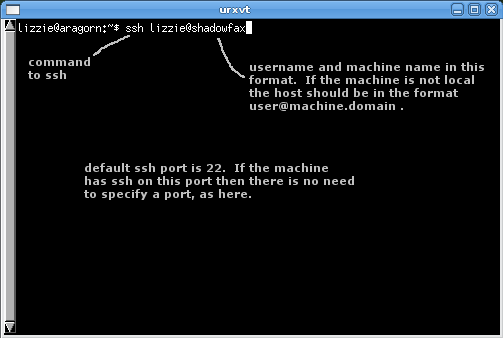
\includegraphics[width=10cm]{figs/terminal.png}
\end{center}


\begin{flushright}
{\tiny
Source: http://carina.org.uk/guidepics/terminal1.png
}
\end{flushright}

\end{frame}



%-----------------------    ---------------------------------

\begin{frame}
\frametitle{SSH}

\begin{center}
  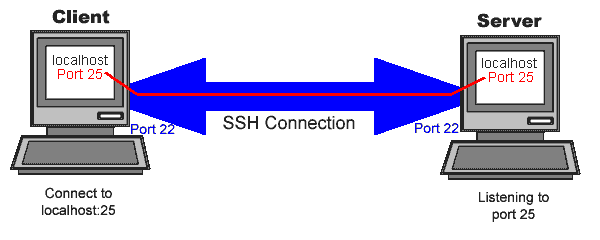
\includegraphics[width=10cm]{figs/ssh-tunnel.png}
\end{center}


\begin{flushright}
{\tiny
Source: http://www.codemastershawn.com/library/tutorial/images/ssh.tunnel.overview.gif
}
\end{flushright}

\end{frame}



\frame{
\maketitle
}

\end{document}
